
\chapter{Responsive Information Visualization}

A \emph{responsive} visualization is a visualization which adapts
itself to the available display space and properties of the device
used to access it. Analogous to responsive web design, the need for
responsive visualizations arises from the growing variety of devices
used to consume content and the physical differences between them.
Visualizations and charts often form significant blocks of content
embedded inside web pages. For a web page to be responsive, any
embedded content such as visualizations and charts must also be
responsive.

Visual elements require proper sizing and spacing to be of
value. Merely scaling visualizations to fit into their allocated space
is insufficient to provide a seamless experience to users, as has
already been discussed in Section~\ref{sec:RWD}. Another factor which
is often ignored is the different methods of interaction inherent to
specific types of devices, such as touch and keyboard interaction. For
example, to ensure that data points remain selectable on less precise
input devices such as touchscreens, a visualisation might adapt by
reducing the data density and increasing the size of individual
elements. The goal of responsive visualizations is that they should
adapt themselves to the characteristics of the consuming device and
context so as to remain as effective and usable as possible
\parencite{DesignPatternsTradeOffsRespVis}.


The topic of responsive visualization only gained prominence in recent
years, as responsive web design became mainstream.
\textcite{BuildingRespDataVisForTheWeb} used the term responsive
visualization, but only descibed how to implement scalable
visualizations. \textcite{LearningRespDataVis} covered scalable
visualizations, but also considered interactive selection and touch
events. \textcite{RespVis} was possibly the first academic work to
address design patterns for responsive visualization.
%
More recently, \parencite{TechniquesForFlexibleRespVisDesign} surveyed
the design space of responsive visualizations, created a taxonomy of
currently used techniques and recurring patterns, and presented a tool
to help design responsive visualisations side-by-side. In addition to
surveying design patterns, \textcite{DesignPatternsTradeOffsRespVis}
also consider issues around different forms of \enquote{message loss}
when reducing chart complexity.





\section{Responsive Visualization Patterns}

Patterns are templates for solving recurring problems.
\textcite{TechniquesForFlexibleRespVisDesign} created a comprehensive
taxonomy of responsive techniques, as well as a tool to help design
responsive visualisations side-by-side. They proposed describing
responsive techniques according to five \emph{actions}, which are
applied to different components. These actions are: (1) resize, (2)
reposition, (3) add, (4) modify and (5) remove. A sixth action refers
to leaving a component unchanged, but this is deemed a non-technique
and therefore left out here. They also described a non-exhaustive set
of eleven \emph{components}, upon which these actions can be
performed: (1) axis, (2) axis labels, (3) axis ticks, (4) gridlines,
(5) legend, (6) data, (7) marks, (8) labels, (9) title, (10) view, and
(11) interaction. It should be noted that some combinations of actions
and components do not make sense and therefore do not occur in
practice. It is, for example, not possible to resize interactions or
reposition data.  \textcite{TechniquesForFlexibleRespVisDesign}
performed their research following a desktop-first approach of
responsive design, because the interviews they conducted with
visualization authors revealed a strong inclination towards this
approach. They found that when adapting desktop visualizations for
narrow screens, it was much more common to remove elements (37.7\%)
than to add them (11.3\%). Another interesting finding was that most
visualizations (88.7\%) implemented no change at all for their
interactions, while some (10\%) even removed interactive capabilities
completely. Only very few visualizations (5.6\%) improved the
experience of mobile users by adapting interactions accordingly.



The most detailed research on patterns in responsive visualization
design was performed by \textcite{DesignPatternsTradeOffsRespVis}.
Following \textcite{TechniquesForFlexibleRespVisDesign}, they
characterised the responsive visualization strategies according to
(the same) two dimensions: \emph{targets}, representing what entity is
changed, and \emph{actions}, representing how entities are changed.
However, the targets and actions are more finely grained, having a
number of sub-categories.
%
Targets are grouped into five distinct categories (Data, Encoding,
Interaction, Narrative, and References/Layout), with four of the five
categories further divided into sub-categories, as shown in
Table~\ref{tab:PatternsTargets}.
%
Actions are also grouped into five distinct categories (Recompose,
Rescale, Transpose, Reposition, and Compensate), with four of the five
top-level categories again having sub-categories, as shown in
Table~\ref{tab:PatternsActions}. The actions are defined as operations
with distinct input and output states to ensure they can be inverted,
and thus can be applied to either desktop-first or mobile-first design
approaches
%
Categorizing techniques using these dimensions, the authors identified
a total of 76 viable strategies, whereby some of them are not used in
the visualizations they studied. However, their explorable online
gallery \parencite{DesignPatternsTradeOffsRespVisGallery} contains
examples demonstrating all these patterns.




% KA need to show the subcategories in the table too!!
% Data:
%   Record
%   Field
%   Level
% etc.

\begin{table}[tp]
\tablestretch
\rowcolors{2}{}{tablerowcolour}
\centering
\begin{tabularx}{\linewidth}{>{\kern-\tabcolsep}lX<{\kern-\tabcolsep}}
\toprule
Category & Description \\
\midrule
Data & Data is the information which is encoded in a visualization. This category includes targets such as data records, data fields, or levels of hierarchy in the data. \\
Encoding & Encodings are the visual forms in which data is represented. \\
Interaction & Interactions define how users can engage with visualizations. This category includes targets such as interaction triggers, interaction feedback and interaction features. \\
Narrative & This category groups targets based on the story a visualization should convey. It contains targets such as the presented sequence of information (views and states) and the information itself in the form of annotations, emphases, and texts. \\
References/Layout & References represent additional information which makes visualizations easier to understand, and a layout describes how the individual visual components are placed. \\
\bottomrule
\end{tabularx}
\caption[Targets of Responsive Visualization Patterns]{
The targets of responsive visualization patterns identified by
\textcite{DesignPatternsTradeOffsRespVis}.
\imgcredit{Table adapted from \textcite{DesignPatternsTradeOffsRespVis}.}
}
\label{tab:PatternsTargets}
\end{table}




% KA need to show the subcategories in the table too!!
% Recompose:
%   Remove
%   Add
%   Replace
%   Aggregate
% etc.

\begin{table}[tp]
\tablestretch
\rowcolors{2}{}{tablerowcolour}
\centering
\begin{tabularx}{\linewidth}{>{\kern-\tabcolsep}lX<{\kern-\tabcolsep}}
\toprule
Category & Description \\
\midrule
Recompose & Actions which affect the existence of targets. Includes remove, add, replace and aggregate actions. \\
Rescale & Actions which affect the size of targets. Includes reduce width, simplify labels and elaborate labels actions. \\
Transpose & Actions which affect the orientation of targets. Includes serialize, parallelize and axis-transpose actions. \\
Reposition & Actions which affect the position of targets. Includes externalize, internalize, fix, fluid and relocate actions. \\
Compensate & Actions which compensate for loss of information. Includes toggle and number actions. \\
\bottomrule
\end{tabularx}
\caption[Actions of Responsive Visualization Patterns]{%
The actions of responsive visualization patterns identified by
\textcite{DesignPatternsTradeOffsRespVis}.
\imgcredit{Table adapted from \textcite{DesignPatternsTradeOffsRespVis}.}
}
\label{tab:PatternsActions}
\end{table}





%% \textcite{RespVisSurvey} have conducted a survey under close
%% supervision by Keith Andrews \parencite{RespVis} identifying nine
%% common patterns which reoccurred in several solutions.  Slightly
%% reworded, these patterns are: (1) rotate axis labels, (2) remove axis
%% ticks, (3) modify strings, (4) transpose chart, (5) reposition
%% components, (6) zoom, (7) filter, (8) modify data density and (9)
%% modify chart type.  Compared to other works, they did not categorize
%% the techniques they found according to multiple dimensions.  Rather
%% than that, they created a collection of specific patterns and, even
%% though they are a good collection on which to base further research,
%% they are not comprehensive enough to cover all the techniques which
%% can be applied to increase the responsiveness of a chart.  An example
%% of a technique which can not be derived from these patterns is the
%% adding and removing of components, such as in the example of a
%% responsive line chart by \textcite{RespVis}, in which the chart's axes
%% were removed on narrow screens.  These patterns also do not consider
%% any adaptations of interactions, which should not be ignored when
%% talking about responsive design.














\section{Responsive Visualization Examples}

% KA you need to gather two or three real-world examples yourself,
% by following the URLs in the responsive-vis-gallery !!

The goal of this section is to provide the reader with some
demonstrative examples of responsive visualizations.  The figures in
this section were taken from external scientific sources which put
most of their effort into demonstrating responsive visualization
patterns rather than communicating messages in the data they used.
Owing to this, some figures below are lacking essential features, such
as titles and axes descriptions, which would usually be present in
practice.


The examples in this section are organized by chart type. It would be
an immense endeavor to bring examples for every pattern used for all
types of charts, so only a subset which demonstrates some of the most
frequently encountered patterns for frequently used types of charts is
summarized here.

% KA introduce a table of the charts by type from Kim et al
% bar     135 35%
% line     98 26%
% scatter  26  7%
% ...

% Where did these numbers come from?
% Did you calculate them yourself?

% The Kim dataset is *not* representative!!
% 280 of 378 charts are from NYT and WSJ.



% Chart prevalence statistics in the wild:
% Reverse-Engineering Visualizations: Recovering Visual Encodings from Chart Images
% Jorge Poco and Jeffrey Heer
% EuroVis 2017
% doi:10.1111/cgf.13193
% https://idl.cs.washington.edu/files/2017-ReverseEngineeringVis-EuroVis.pdf







\subsection{Bar Charts}

Bar charts are very widespread, accounting for 135 (= 36\%) of the 378
responsive charts in the corpus collected by
\textcite{DesignPatternsTradeOffsRespVis}. Bar charts are usually used
to visualize two-dimensional data, with one categorical dimension and
one quantitative dimension. Two variants of bar charts support the
visualization of categorical datasets having subdimensions: grouped
bar charts \parencite{GroupedBar} compare subdimensions with each
other, and stacked bar charts \parencite{StackedBar} compare
part-to-whole relationships of the subdimensions. Even though
responsive design of visualizations is slowly becoming more common,
most charts found in today's web articles are still created as static
images \parencite{HBar,VBar,HVBar,MapBarLine}.

A good example of a responsive bar chart can be seen in
Figure~\ref{fig:RespBarExample} \parencite{RespVis}. Bar charts are
freely scalable by adjusting the width of individual bars
\parencite{RespHBar,RespHBarHLine,RespHBars}, so they all can fit into
their allocated space. When reducing the width of any type of chart
past a certain point, the tick labels of the horizontal axis may start
to overlap. This is why the reducing width pattern usually occurs
together with the recompose axis ticks and simplify/elaborate axis
labels patterns \parencite{RespHBars,RespHBarHLine,RespVBar}. Another
effective pattern for avoiding overlapping tick labels is to rotate
the labels by up to 90 degrees tso they take up less horizontal space
\parencite{RespVis}. If there is too much data to fit into the
available width, the chart can be transposed and grown to as much
height as is required necessary \parencite{RespVis}. Doing this is
more advisable than simply extending the width of the chart past the
viewport, since vertical scrolling is easier than horizontal
scrolling. When reducing the width of charts containing annotations, a
number of patterns can be applied to avoid annotations
overlapping. For example, annotations can be removed
\parencite{RespHStackedBar,RespHLineHStackedBar}, simplified, or
relocated \parencite{RespVBar}.



\begin{figure}[tp]
\newlength{\respbarwidth}
\setlength{\respbarwidth}{0.95mm}
\centering
\subfloat[][%
70rem
]
{%
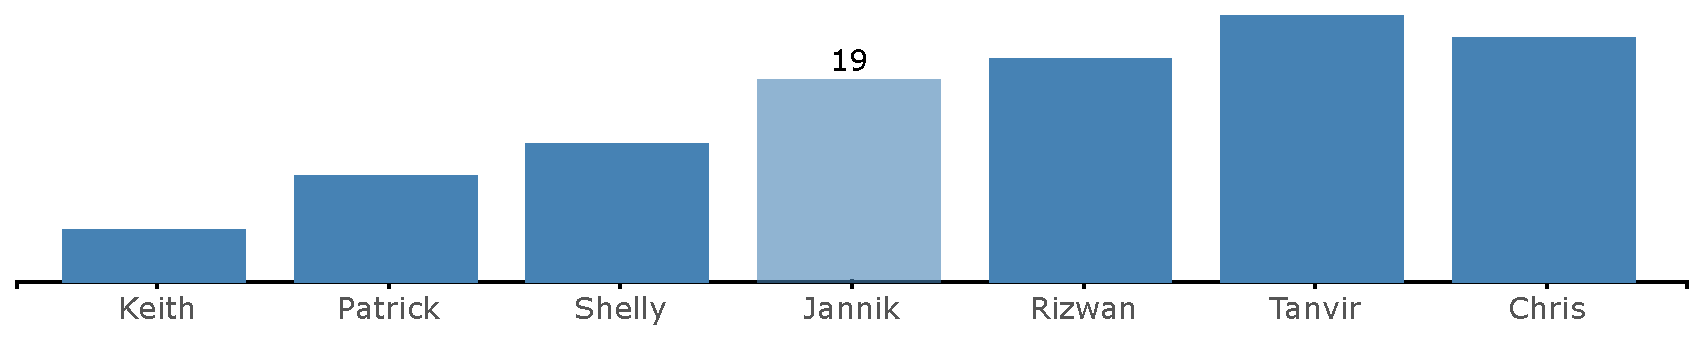
\includegraphics[width=70\respbarwidth]
{diagrams/resp-bar-1.pdf}%
\label{fig:RespBarExample1}%
}
\hfill
\subfloat[][%
50rem
]
{%
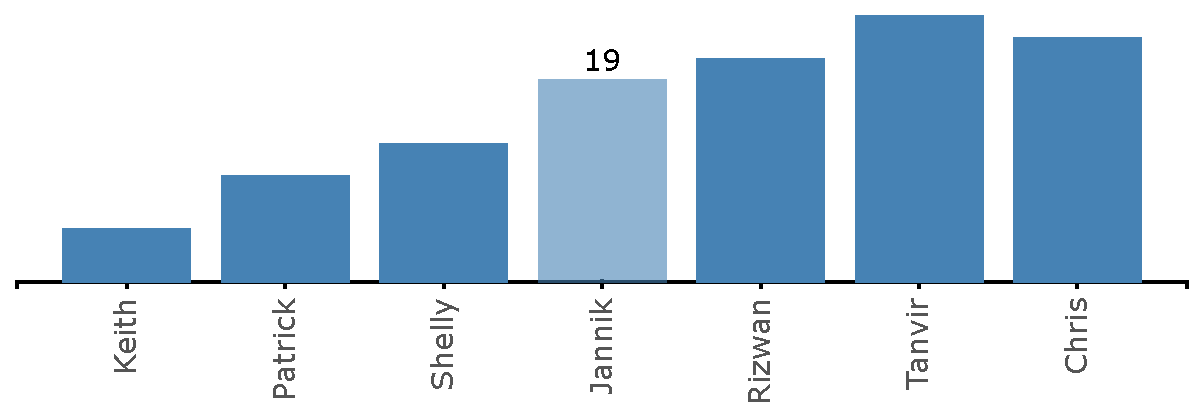
\includegraphics[width=50\respbarwidth]
{diagrams/resp-bar-2.pdf}%
\label{fig:RespBarExample2}%
}
\hfill
\subfloat[][%
30rem
]
{%
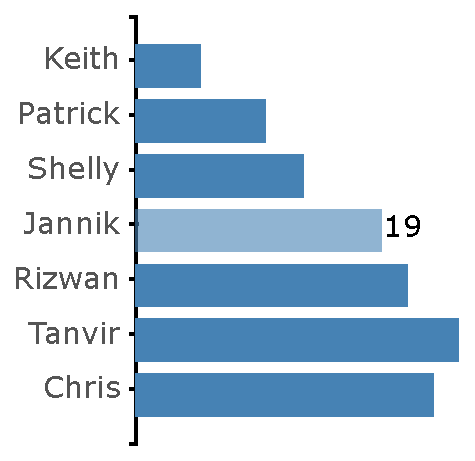
\includegraphics[width=30\respbarwidth]
{diagrams/resp-bar-3.pdf}%
\label{fig:RespBarExample3}%
}
\caption[Responsive Bar Chart Example]
{
An example of a responsive bar chart at different display widths.
\subref{fig:RespBarExample1} At 70rem, axis tick labels are aligned
horizontally. \subref{fig:RespBarExample2} At 50rem, axis tick labels
are aligned vertically. \subref{fig:RespBarExample3} At 30rem, the
chart is transposed.
\imgcredit{Screenshots of \textcite{RespVis} created by the author of
  this thesis. Used with kind permission by Keith Andrews.}
}
\label{fig:RespBarExample}
\end{figure}






\subsection{Line Charts}

The second most frequent type of responsive charts according to the
responsive visualization gallery
\parencite{DesignPatternsTradeOffsRespVis} are line charts, which
number 98 (= 26\%) out of the 378 responsive visualizations in the
gallery. Line charts are used to show trends in two-dimensional
datasets by plotting them as points connected by lines (a polyline).
They can be extended to compare trends in an additional categorical
dimension by drawing additional polylines for each category. Many line
charts on the web are published in non-responsive forms
\parencite{HLine,HLine2}, although some authors take the extra effort
to make their charts responsive. The minimum which can be done to make
a line chart responsive is to reduce their width
\parencite{RespRadialScatterHLine} on narrower screens by shrinking
the horizontal distance between neighboring points. This usually
occurs together with the recomposition and simplification of
horizontal ticks. If the chart contains annotations, it may also be
necessary to recompose, relocate, and simplify them as well
\parencite{RespHLines,RespHLine,RespHBarHLine,RespHLineHStackedBar}.

A good demonstration of which responsive patterns can be applied to
make a line chart responsive is shown in the responsive line chart
created by \textcite{RespVis} which can be seen in
Figure~\ref{fig:RespLineExample}. In addition to the recomposition of
ticks, tick labels are rotated to reduce their required horizontal
space. For exceptionally limited space, it can make sense to remove
the axes of a line chart entirely and turn it into a sparkline.
% KA Need a bib entry and ref to sparkline
However, it should be noted that by doing this, the consumer of the
visualization loses information about the type and scale of the
chart's dimensions. This technique should therefore only be applied in
cases where no other pattern is applicable or if the trend in the data
is the most important message to convey. It is rare to encounter
transposed versions of line charts, although transposition could
sometimes benefit heavily annotated line charts
\parencite{VLine}. Applying a transpose pattern would allow the chart
to take up as much vertical space as necessary to neatly accomodate
annotations without requiring the consumer to scroll horizontally.



\begin{figure}[tp]
\newlength{\resplinewidth}
\setlength{\resplinewidth}{1.15mm}
\centering
\subfloat[][%
65rem
]
{%
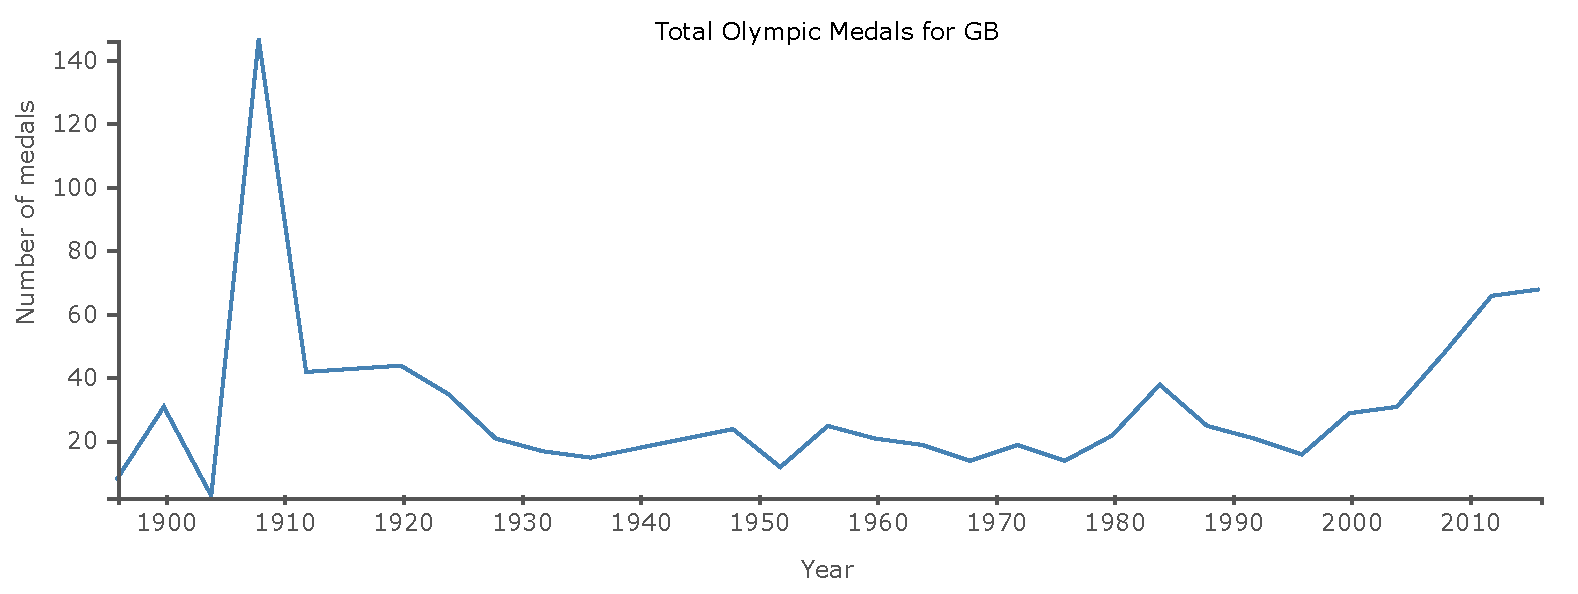
\includegraphics[width=65\resplinewidth]
{diagrams/resp-line-1.pdf}%
\label{fig:RespLineExample1}%
}
\hfill
\subfloat[][%
40rem
]
{%
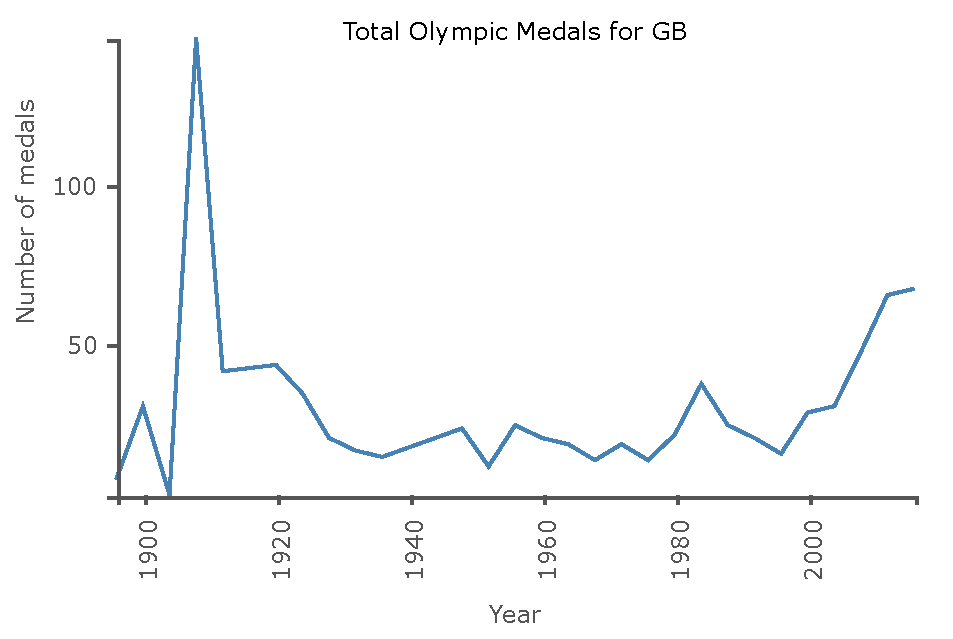
\includegraphics[width=40\resplinewidth]
{diagrams/resp-line-2.pdf}%
\label{fig:RespLineExample2}%
}
\hfill
\subfloat[][%
20rem
]
{%
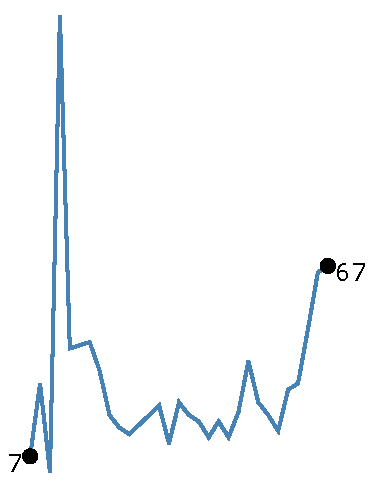
\includegraphics[width=20\resplinewidth]
{diagrams/resp-line-3.pdf}%
\label{fig:RespLineExample3}%
}
\caption[Responsive Line Chart Example]
{
An example of a responsive line chart at different display widths.
\subref{fig:RespLineExample1} At 65rem, the x axis labels are
horizontal.  \subref{fig:RespLineExample2} At 40rem, the x axis ticks
have been thinned out and the labels fully rotated by 90\textdegree.
\subref{fig:RespLineExample3} At 20rem, both axes have been removed,
and the chart has become a sparkline.
\imgcredit{Screenshots of \textcite{RespVis} created by the author of
  this thesis. Used with kind permission by Keith Andrews.}
}
\label{fig:RespLineExample}
\end{figure}









\subsection{Scatterplots}

Scatterplots are also quite frequently encountered among responsive
charts, numbering 26 (= 7\%) of the 378 responsive charts contained in
the gallery by \textcite{DesignPatternsTradeOffsRespVis}. A
scatterplot represents two-dimensional data as points in a 2d
Cartesian coordinate system. There are many examples of scatterplots
published as static images \parencite{Scatter,Scatter2}, with
responsive versions starting to emerge.

The first step to making scatterplots responsive is to reduce their
width to fit them into the space available. As for other types of
chart, care must be taken to avoid overlapping of labels and
annotations by applying recomposition, relocation and simplification
patterns \parencite{RespScatter,RespScatter2}. To counteract the
increased density of points when reducing the size of their container,
various interaction features are usually implemented in scatterplots
which help consumers in making sense of the represented data. The most
useful interaction features in these charts are elaborative zooming
interactions and the explorative panning interactions. In addition to
zooming and panning, \textcite{RespVis} employs additional methods to
ameliorate the overlapping of individual points, including fisheye
distortion, Cartesian distortion, and temporary displacements of
points.

An interesting technique for responsive scatterplots based on the
visualization's density (data points per pixel) rather than its width
was introduced by \textcite{NickRabinowitzRDV}. The benefit of this
approach is that charts adapt to changing amounts of data and
reconfigure their appearance accordingly. The patterns applied in the
responsive scatterplot shown in Figure~\ref{fig:RespScatterExample}
are the recomposition of annotations to only show annotations for
selected data records, and the switching of the encoding from a
scatterplot to a heatmap for high point densities. Other techniques,
such as the recomposition of data records, would also be applicable to
responsive scatterplots, but no examples for such patterns could be
found. If the data to be encoded is inherently cyclic, a radial
scatterplot, using polar coordinates, can be used to better reflect
the cyclic nature of the data \parencite{RespRadialScatterHLine}.



\begin{figure}[tp]
\centering
\subfloat[][%
Small number of data points. % (0.00005 points per pixel).
]
{%
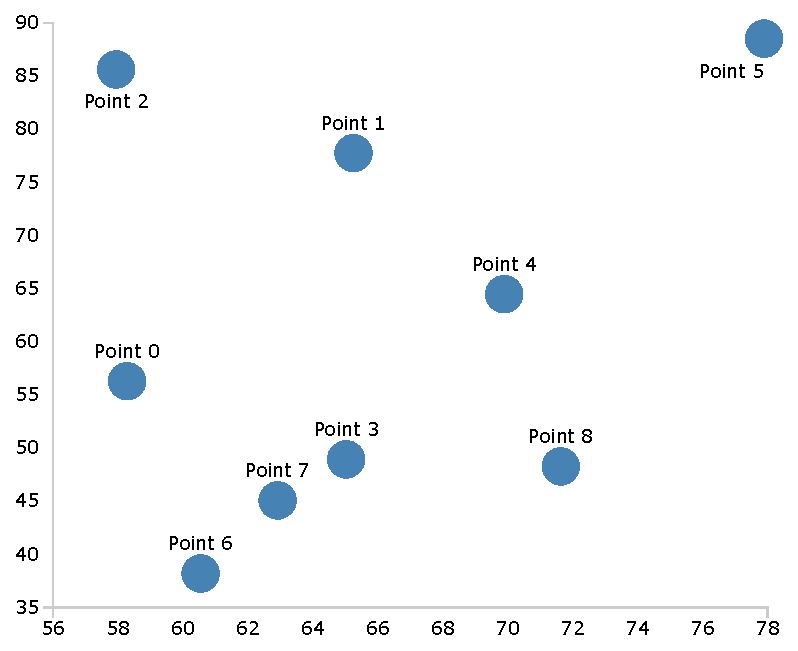
\includegraphics[width=0.3\linewidth]
{diagrams/resp-scatter-1.pdf}%
\label{fig:RespScatterExample1}%
}
\hfill
\subfloat[][%
Medium number of data points. % (0.0007 points per pixel).
]
{%
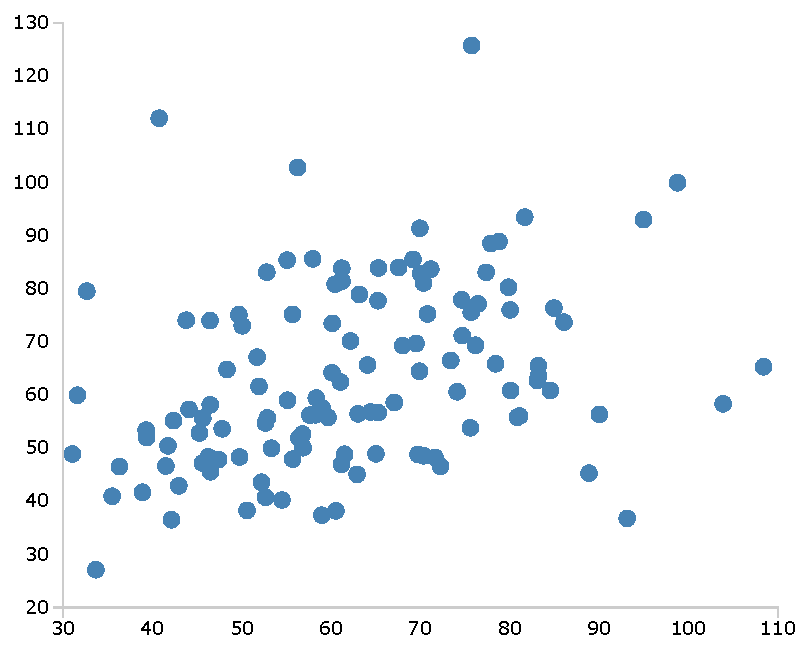
\includegraphics[width=0.3\linewidth]
{diagrams/resp-scatter-2.pdf}%
\label{fig:RespScatterExample2}%
}
\hfill
\subfloat[][%
Large number of data points. % (0.017 points per pixel).
]
{%
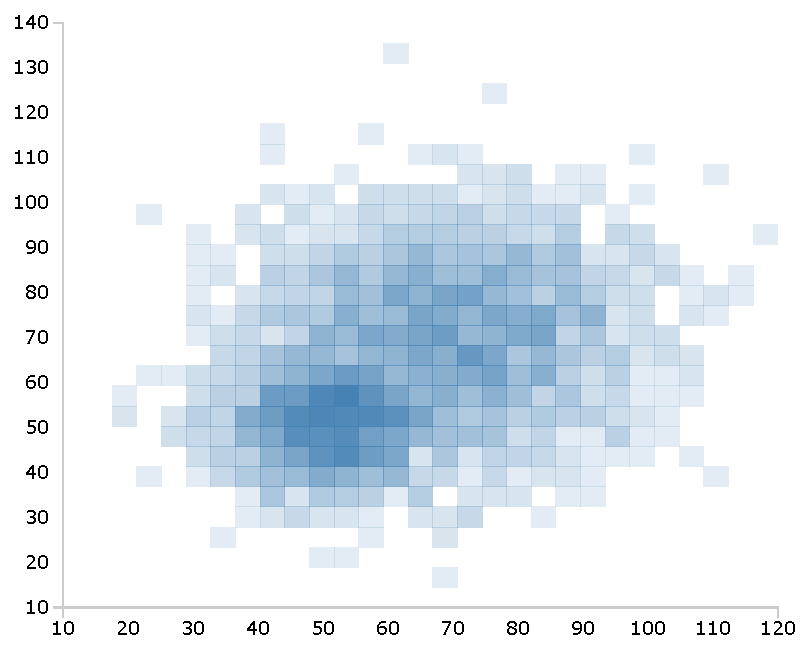
\includegraphics[width=0.3\linewidth]
{diagrams/resp-scatter-3.pdf}%
\label{fig:RespScatterExample3}%
}
\caption[Responsive Scatterplot Example]
{
An example of a responsive scatterplot based on data density (data
points per pixel). \subref{fig:RespScatterExample1} With a small
number of data points, all points and their corresponding labels are
shown. \subref{fig:RespScatterExample2} At a certain density, labels
are only shown for selected points. \subref{fig:RespScatterExample3}
At very large densities, the scatterplot is replaced by a heatmap to
more efficiently display the large amount of data.
\imgcredit{Screenshots created by the author of this thesis.
Visualization created by \textcite{NickRabinowitzRDV}}
}
\label{fig:RespScatterExample}
\end{figure}








\subsection{Parallel Coordinates}

% KA  How many and % in Kim dataset?

% include Ref to Alfred Inselberg book

Even though parallel coordinates charts are rarely encountered in
non-technical contexts, they are very popular when it comes to
visualizing multidimensional data in visual analytics systems
\parencite{HighD}. In these kinds of charts, multiple dimensions are
rendered as parallel axes, upon which points are connected via paths
(polylines). Each polyline represents a data record and its values at
the corresponding dimensions. The axes of a parallel coordinates chart
are typically laid out horizontally, meaning that the chart can be
made narrower by reducing the distance between individual axes.
Previously mentioned axis-related responsive patterns, such as
rotating labels and recomposing ticks, can also be applied.

Another technique is to temporarily hide some dimensions, based on
some criteria. When automatically hiding dimensions, it is necessary
to apply compensation patterns, giving the user additional controls to
configure which dimensions are displayed and override the system's
hiding behavior. An example of a responsive parallel coordinate chart
incorporating some of these patterns can be seen in
Figure~\ref{fig:RespParCoordExample}.
%
If reducing the chart's complexity is not appropriate, an alternative
is to transpose the chart, so its dimensions are laid out vertically
and vertical scrolling can be used to explore the full chart.




\begin{figure}[tp]
\newcommand{\respparcoordscale}{0.36}
\centering
\subfloat[][%
61rem
]
{%
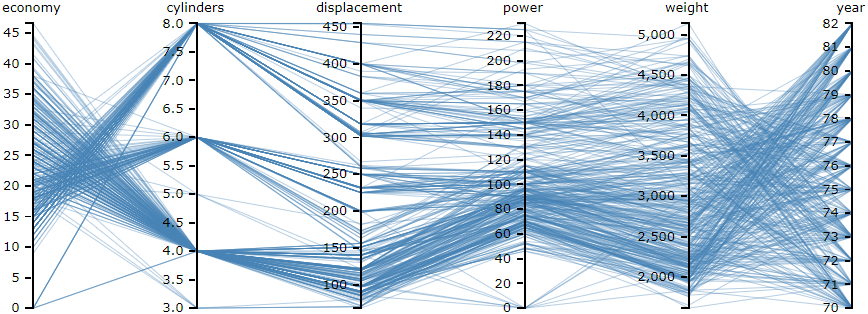
\includegraphics[valign=b,scale=\respparcoordscale]
{images/resp-parcoord-1.png}%
\label{fig:RespParCoordExample1}%
}
\hfill
\subfloat[][%
50rem
]
{%
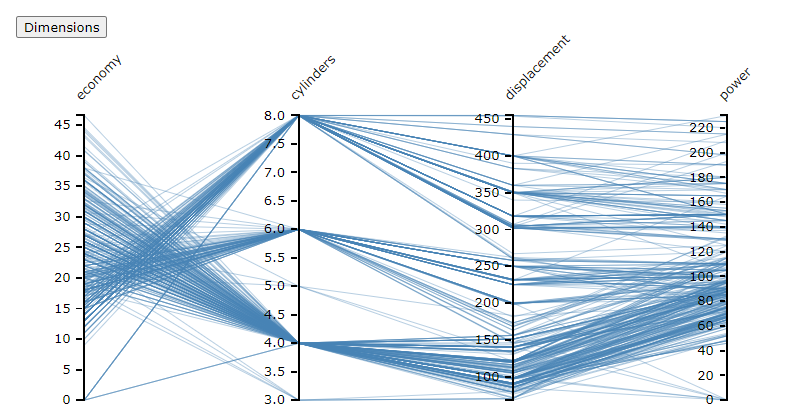
\includegraphics[valign=b,scale=\respparcoordscale]
{images/resp-parcoord-2.png}%
\label{fig:RespParCoordExample2}%
}
\newline
\subfloat[][%
40rem
]
{%
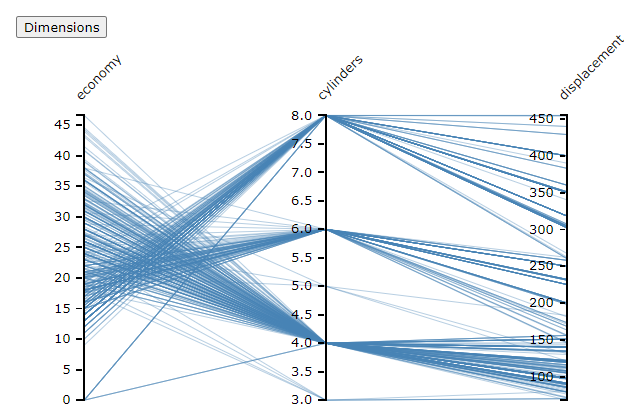
\includegraphics[valign=b,scale=\respparcoordscale]
{images/resp-parcoord-3.png}%
\label{fig:RespParCoordExample3}%
}
\hfill
\subfloat[][%
30rem
]
{%
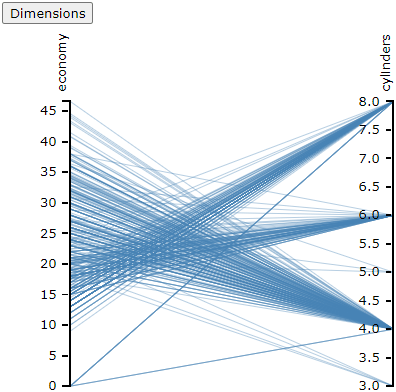
\includegraphics[valign=b,scale=\respparcoordscale]
{images/resp-parcoord-4.png}%
\label{fig:RespParCoordExample4}%
}
\hfill
\subfloat[][%
30rem, user-configured dimensions
]
{%
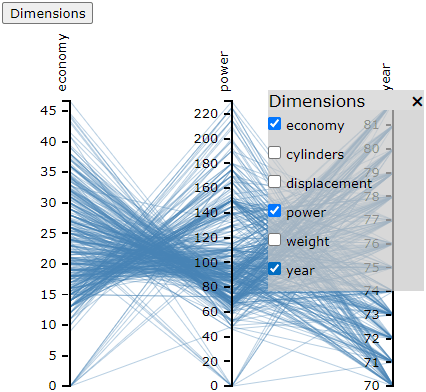
\includegraphics[valign=b,scale=\respparcoordscale]
{images/resp-parcoord-5.png}%
\label{fig:RespParCoordExample5}%
}
\caption[Responsive Parallel Coordinates Chart Example]
{
A responsive parallel coordinates chart at different display widths.
\subref{fig:RespParCoordExample1} At larger widths, all dimensions are
shown. \subref{fig:RespParCoordExample2} Dimensions are removed based
on their priority, dimension labels are rotated by 45 degrees, and a
dimensions toggle is shown which enables the configuration of
dimensions. \subref{fig:RespParCoordExample3} Further dimensions are
removed. \subref{fig:RespParCoordExample4} Further dimensions are
removed, and dimension labels are rotated by 90 degrees.
\subref{fig:RespParCoordExample5} The dimension configuration panel
has been opened, and the user has taken control over which dimensions
to show.
\imgcredit{Screenshots of \textcite{RespVis} created by the author of this thesis.
Used with kind permission by Keith Andrews.}
}
\label{fig:RespParCoordExample}
\end{figure}

